\documentclass[10pt,twocolumn]{article} 

% use the oxycomps style file
\usepackage{oxycomps}

% read references.bib for the bibtex data
\bibliography{references}

% include metadata in the generated pdf file
\pdfinfo{
    /Title (Tutorial Report)
    /Author (Sammy Sanchez)
}

% set the title and author information
\title{Tutorial Report}
\author{Sammy Sanchez}
\affiliation{Occidental College}
\email{sanchezs@oxy.edu}

\begin{document}

\maketitle

\begin{abstract}

This tutorial teaches a person how to match basketball player IDs between different databases and in other words deduplicate the players between the sources. The reason that this tutorial can be useful is when a player's name is different between the database sources and a the user wants to match that person's stats between the databases. To achieve this tutorial, you have to parse the data to find the data that matches between the sources and it will map the ids between the sources. The tutorial is written by Ryan \textcite{Tutorial} on GitHub.

\end{abstract}

\begin{abstract}

This tutorial teaches a person how to match basketball player IDs between different databases and in other words deduplicate the players between the sources. The reason that this tutorial can be useful is when a player's name is different between the database sources and a the user wants to match that person's stats between the databases. To achieve this tutorial, you have to parse the data to find the data that matches between the sources and it will map the ids between the sources. The tutorial is written by Ryan \textcite{Tutorial} on GitHub.

\end{abstract}

\section{Methods}
The methods for this tutorial is using Python to do the programming. You have to import 4 libraries for this tutorial to work and they are:

\begin{itemize}
    \item Pandas 0.23.4
    \item urllib 1.24.1
    \item BeautifulSoup4 4.6.3
    \item fuzzywuzzy 0.17.0
\end{itemize}

The first step of this tutorial is to get the player data from the website \url{stats.nba.com} and the code uses the pandas and urllib3 libraries and I picked the basketball season 2018-19. Then you make a function that extracts the data from the website. It parses the data and converts the objects into a dataframe. The last thing that happens in the function is that the column names are set for the data and the data is saved to a csv file.

The second step for this tutorial is obtaining the basketball data from \url{https://www.basketball-reference.com/}. This part of the code uses the bs4, urllib3 and pandas libraries. The urllib3 library gets the page, bs4 library parses the html and pandas will store the data. Next we set the season to 2019 and initialize an array the is the table and an array for the columns. Then we create a process to request the page on the website and parse the page to extract the column names and the data in the rows. Then we will convert this to a dataframe. Next, there is a function to extract the column names and store them in an array and doing another function for the rows and parsing them for the data. Parsing the rows will get the player id which is what we need so we can compare this website with stats.nba.com and it will also find the anchor tag in the player name. Once the table from these functions are in the dataframe, we set the column names and save them to a CSV file.

The last step to this tutorial is using the data that was parsed and stored to generate a table with the player id of each source and make them matching the specific player. The data that is used to be compared between the sources are assists, filed goal attempts and rebounds. The libraries used are fuzzywuzzy and pandas. Fuzzywuzzy compares the fuzzy strings and pandas reads the csv files and joins them. The first step is to read out the data from both website's csv files and convert the player id to a string. Then we have to map a single season for stats.nba because it is two years of data and we need it to match basketball reference's one year of data. Next was deduplicating the data from basketball reference for the selected stats stated earlier and do the same for stats.nba for the stats to match. Next there has to be a join between the two dataframes created. With this join, it will match the data from both files and the only columns that remain are the player's name and id columns from both sources. With this join, you have to handle the cases where there was no exact data matches and it takes the rows that have null values and separate the frame back into the original data files from the websites. Then we join the data again, but not with the player name as a condition for the join statement and see if the rebounds, assists and field goal attempts match up. Next, we check if the fuzzy name match ratio is higher than 60\% to have accurate data to match and then we merge the fuzzy matches with the exact matches and save the results to a csv file. 

This tutorial should have produce the csv file to have the name of the player from basketball reference and the id used on the website and the name of the player from stats.nba and the id used on the website. This would be good for people who want to know how to match basketball statistics between sources and find out how a player is referenced with a specific id given to them in the website database. In Figure 1, it show what the results look like after completing the tutorial with the desired outcome of matching the player ids between two sources.

\begin{figure}
    \centering
    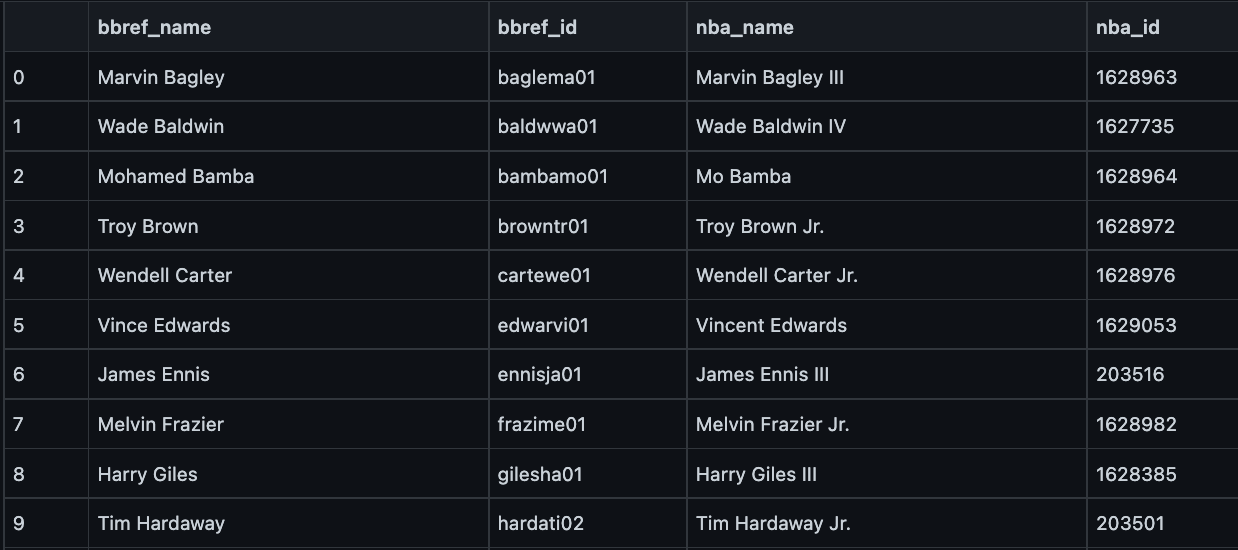
\includegraphics[width=.95\linewidth]{results.png}
    \caption{
       Results from the Tutorial
    }
    \label{fig:first-page}
\end{figure}
 
\section{Evaluation}

The results of this tutorial shows that it worked comparing player stats between two different sources and finding the player id associated with each website. This is crucial for people trying to query data from different sources because of how a player's name can be different in each website. As show in Figure 1, Troy Brown's name is different in basketball reference compared to stats.nba which uses Troy Brown Jr. as the name. This tutorial would be useful for people that try to use specific player names to gather data and it could fail if they do not get the string 100\% accurate. For my project, having these player ids can be crucial to collecting data because there would not be any errors since the strings of the names of player could potentially cause those errors. I evaluated this tutorial based on how well the code I followed ran correctly and was able to store the data I wanted to compared accurately. The players that the query resulted in had no errors with the name matching even though some of the players had slightly different names, mostly with a Jr. at the end of a hyphen in their last name. To know this tutorial worked is also how the data collected from each website database had matching strings or the stats that were queried from them. The table would have never join correctly if the stats collected from each website were off and not the same. You can look at the csv file created for basketball reference and the other csv file created by the stats.nba and manually check the player and their stats to see a match to make sure the accuracy of the code was correct. To also evaluate this tutorial, the user can change the stats to be compared when gathering the data from the websites. Instead of field goal attempts, rebounds and assists, it can be changed to points scored, three pointer made and steals. Then you can make the results from the websites into two more csv files and compare them and join to see if the same results appear. This will show how accurate the tutorial would be even with different stats used to see if it can compare the player ids and names between the websites. 

\section{Discussion}

This tutorial teaches users how to extract data from different sports statistic websites despite teaching the user how to match player id with potentially different names. Knowing how to extract data using specific parameters with the stats being parsed is big for a project that wants to use statistics in charts and graphs. Knowing how to query a table of data is also important for collecting specific statistics that the user wants to use for their project. This can be applied to any website that contains data and can be used for research or projects to help the user obtain what he wants. Sports analysts most likely use queries to find specific points of data to write about and analyze when discussing what draft prospect they see the most potential in or how MVP voting is influence based on the stats chosen. The people can extract certain data for their research and learning how to do so with queries helps them pinpoint it better than just looking at a database with a bunch of different statistics in a chart or table. 

Some ethical issues with this tutorial can be how the data is used to spread misinformation about players with certain stats that are seen as negative because social media is known to berate sports players for bad performances. If someone were to use part of this tutorial to find stats that negatively represent a player and share it to social media, it can influence others to go after that player and possibly make negative or threatening comments towards them. Another ethical issue could be how a player's stats are used for gambling purposes and influencing people to bet on a player when stats can be misleading. If someone were to query specific stats and influence others to gamble on that player getting the stat for the night, it can potentially be misleading and cause people to lose money with that influence. 

Despite some problems that this tutorial might create, it was very effective of matching player's names and their ids between different websites and has potential to go further with making sure the stats are accurately portrayed and querying data that will be useful for the user like specific stats. Finding data that might be out of the ordinary like year born or percent of 3 pointers in a year can be used to compare players and find unique results. It can help influence a creation of a new statistic that is measured with combined stats that the user picks. 

\printbibliography 

\end{document}
